\chapter{Introduction}

\section{Overview}

\texttt{permute} is a Python library for permutation tests and confidence sets.
Philip B. Stark, Kellie Ottoboni, and I developed this package over the
last year with most of the work occurring over the last few months.
Here are a few relevant links for the project:
\begin{itemize}
\item Website (including documentation): \url{http://statlab.github.io/permute}
\item Mailing list: \url{http://groups.google.com/group/permute}
\item Source: \url{https://github.com/statlab/permute}
\item Bug reports: \url{https://github.com/statlab/permute/issues}
\end{itemize}
In this report, I will briefly explain the purpose of the package, our
development practices, the currently available functionality, and
our immediate and long-term roadmap.

\subsection{Permutation tests}

Permutation tests provide a non-parametric approach to hypothesis testing.

Permutation tests and confidence sets for a variety of nonparametric testing
and estimation problems, for a variety of randomization designs.
   
Test statistics in each stratum ...

Methods of combining tests across strata ...

Nonparametric combinations of tests ...

\subsection{Confidence sets}

\subsection{Python}

Python is a high-level, general purpose programming language, which has
become increasingly popular for scientific computing
\cite{millman2011python, Perez2011}. Unlike most high-level languages
used in scientific computing, Python was not specifically designed for
scientific applications.  However, it quickly attracted interest among
scientists and engineers.  Initially, it was primarily employed as ``glue''
language to couple together low-level numeric libraries written in C or
Fortran with high-level scientific application languages such as Matlab.

In addition to standard Python, \texttt{permute} makes heavy use of
of third-party libraries NumPy\footnote{\url{http://numpy.org}} and
SciPy\footnote{\url{http://scipy.org}}.

NumPy is

Mersenne Twister
624-vector of 32-bit integers

SciPy
for optimization functions such as Brentq and statistics functions.


\section{Development practices}

As this is a new software project, we invested a significant effort in
setting up a development infrastructure to ensure that all our work
is carefully tracked and thoroughly and continually tested.  In particular,
we have adopted and implemented many of the best software practices
employed by many successful open source software projects \cite{millman2014}.

\subsection{Version control}

We are using Git\footnote{\url{http://git-scm.com}} as our version control
system and GitHub\footnote{\url{https://github.com}} as the public hosting
service for our official \texttt{upstream} repository.

\subsubsection{Workflow}

Rather than work on the \texttt{master} branch of our repositories,
we have adopted the policy of performing all code changes on
feature branches.

\subsubsection{Pull requests}

To get new code integrated in the official \texttt{upstream} master, we use
GitHub's \emph{pull request} mechanism.  This helps make performing code review
for new code added to the official ``upstream'' repository easy to manage.
Given the short development history and the fact that there is only one
developer adding most of the code, we have 

\subsection{Testing}

We use the \texttt{nose} testing framework for automating our testing
procedures.\footnote{\url{https://nose.readthedocs.org}}  This is the
standard testing framework used by most of the core packages in
the scientific Python ecosystem.

For example, from the top-level of the repository, you can ask \texttt{nose}
to run the tests by entering \texttt{nosetests permute} in Bash.  For example,

\begin{verbatim}
$ nosetests permute 
......................................................................
----------------------------------------------------------------------
Ran 35 tests in 37.923s
\end{verbatim}

In the above console output, you will see a ``.'' for each test, which
is run.  A test corresponds to a function and each test may test several
things.

\subsubsection{Coverage}

We also use \texttt{nose} to monitor our test coverage.  Our goal is to
test everyline of code.  For example, not only do we want to test every
function in our package, but if a specific function has internal logic
we want to test each possible path through the function.  Having tested
each line of code increases our confidence in our codebase, but more
importantly provides us assurance that changes we make do not break
existing code.

Working in the top-level of our local repository in Bash, you could
enter

\begin{verbatim}
$ nosetests permute --with-coverage --cover-package=permute
Name                 Stmts   Miss Branch BrMiss  Cover   Missing
----------------------------------------------------------------
permute                 43      7     10      2    83%   72, 77-88, 113
permute.core            55      0     30      4    95%   
permute.data            45      0      2      0   100%   
permute.eda             22      0      8      0   100%   
permute.irr             52      0     20      2    97%   
permute.stratified      44      0     16      4    93%   
----------------------------------------------------------------
TOTAL                  261      7     86     12    95%   
----------------------------------------------------------------------
Ran 35 tests in 39.985s
\end{verbatim}
Here you can see, that in addition to running 35 tests without error,
that over 95\% of our code has at least one test.

\subsubsection{Continuous integration}

Travis CI\footnote{\url{https://travis-ci.org}}


\texttt{coveralls}\footnote{\url{https://coveralls.io}}

\begin{figure}
  \begin{centering}
    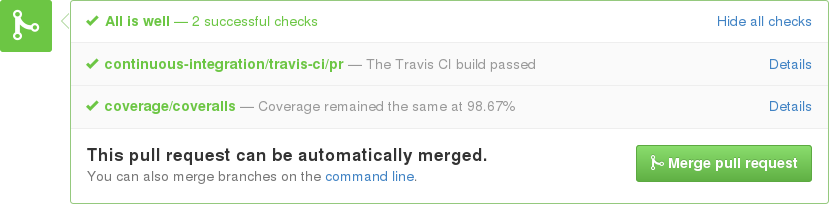
\includegraphics[width=5.5in]{fig/pull-request-ci.png}\par
  \end{centering}

  \caption{\label{fig:pull-request}Pull request and continuous integration.}
\end{figure}

\subsection{Documentation}

Docstring standard \cite{SciPyProceedings_27}.

ReStructured Text

\texttt{sphinx}
